\newpage

\section{Lines in Triangles}

\begin{teachingnote}
This activity is first about the meanings of median, altitude, angle bisector, and perpendicular bisector.  Then it is about noticing that they are four different lines in a general triangle.  
\end{teachingnote}

Two copies of a triangle are shown below.   In each triangle, \textbf{draw carefully} the designated lines.  \emph{You do not need to construct these lines:  careful measurements are allowed.}

\begin{prob}
In the triangle on the left, draw the median from $B$ to $\overline{AC}$, the altitude from $B$ to $\overline{AC}$, the angle bisector of $\angle B$, and the perpendicular bisector of $\overline{AC}$.  

%\begin{enumerate}
%\item Median from $B$ to $\overline{AC}$
%\item Altitude from $B$ to $\overline{AC}$
%\item Angle bisector of $\angle B$
%\item Perpendicular bisector of $\overline{AC}$
%\end{enumerate}
\end{prob}

\begin{prob}
In the triangle on the right, draw the median from $C$ to $\overline{AB}$, the altitude from $C$ to $\overline{AB}$, the angle bisector of $\angle C$, and the perpendicular bisector of $\overline{AB}$. 

%\begin{enumerate}
%\item Median from $C$ to $\overline{AB}$
%\item Altitude from $C$ to $\overline{AB}$
%\item Angle bisector of $\angle C$
%\item Perpendicular bisector of $\overline{AB}$
%\end{enumerate}
%
\end{prob}

\begin{prob}
In each triangle, you should have drawn four different lines.  What can you say about a triangle for which two or more of these lines turn out to be the same?  
\end{prob}

\vfill
\begin{fullwidth}
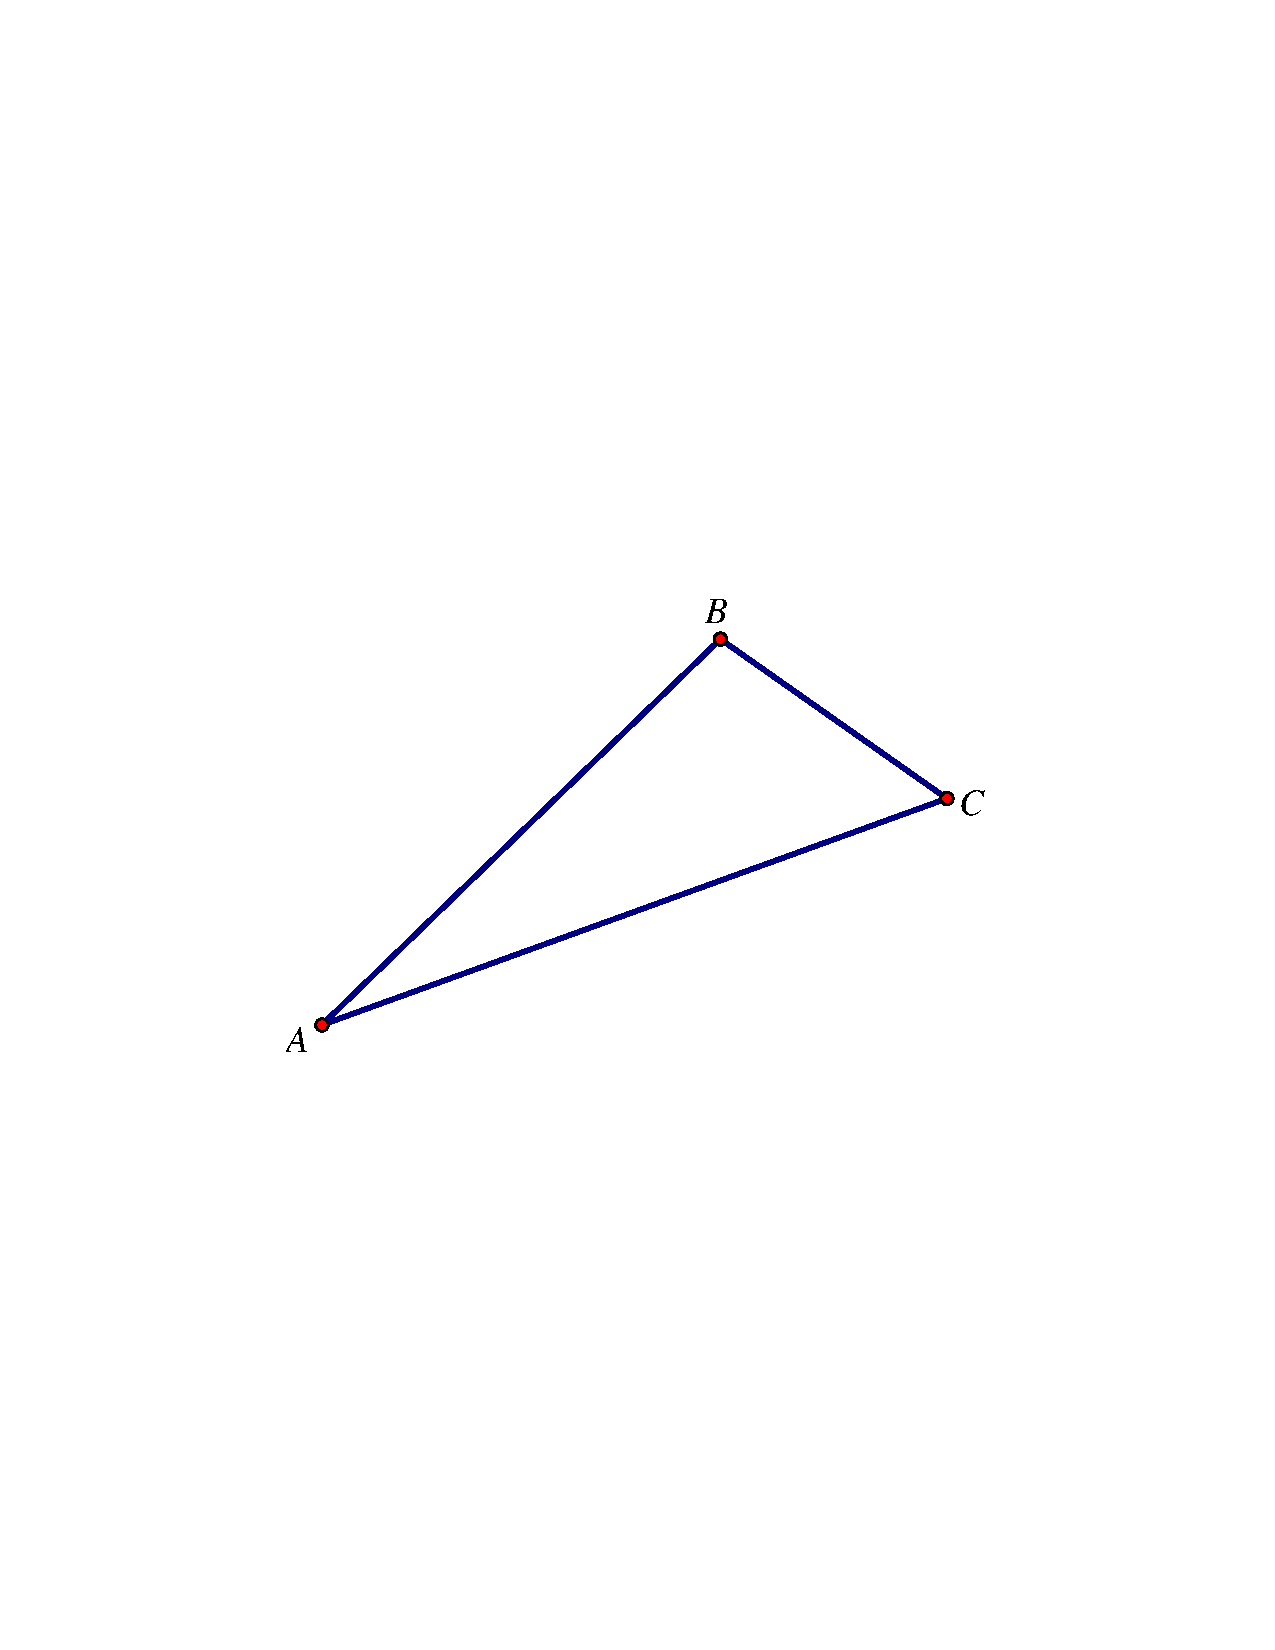
\includegraphics[scale=0.9]{../graphics/obtuseTriangle.pdf}
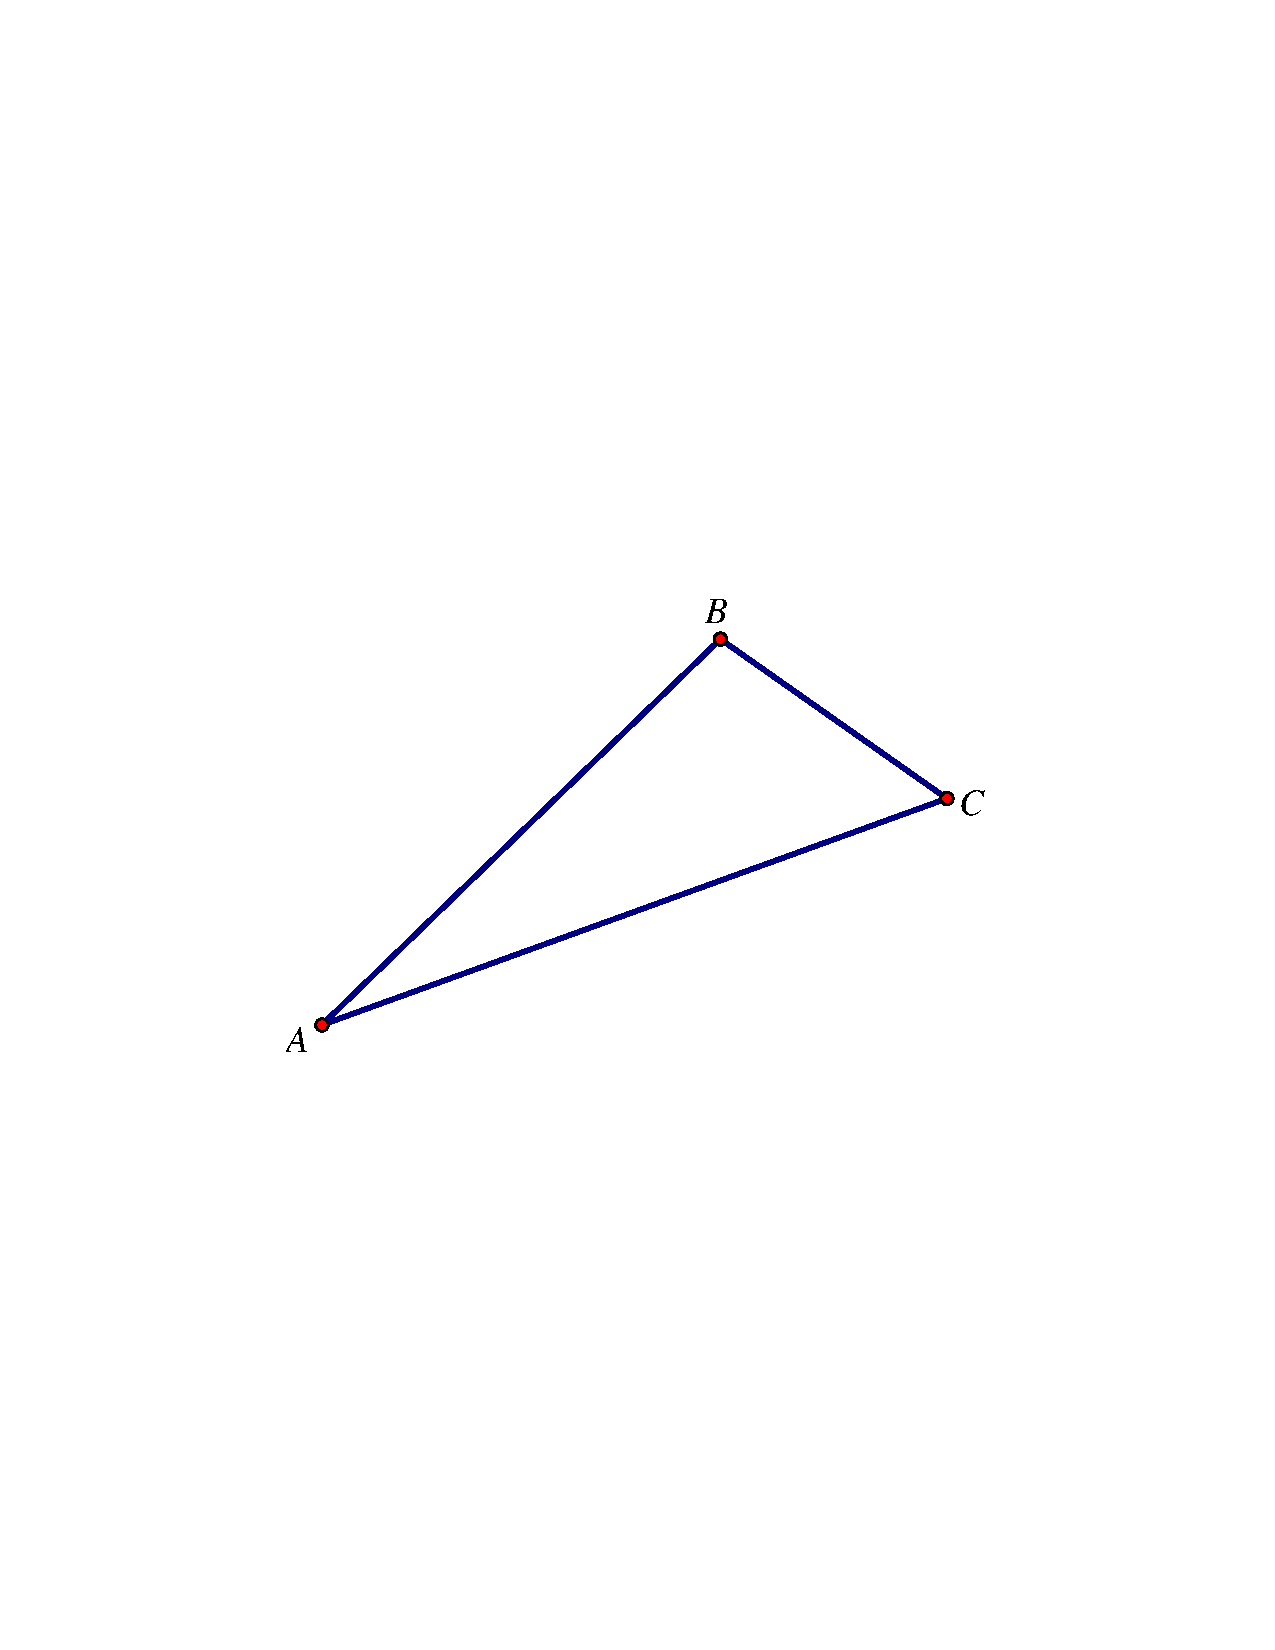
\includegraphics[scale=0.9]{../graphics/obtuseTriangle.pdf}
\end{fullwidth}

\vfill
